\section{Expressions}
\label{sec:Expressions}
This part of the language describes expressions. Expressions are in The Language Described in This Report defined as the constructs that have a value. These can be used together with specific operators to create larger expressions as one would do in mathematics. Apart from combining expressions they are often used as the right hand side of an assignment, but can also be used for indexing, the condition in conditional statements, for return values and in general all places where a value is expected.

First we look at the mathematical operators that can combine expressions.
\setlength{\grammarindent}{100pt}
\begin{grammar}
<Operation> ::= <Operation> <PSIXOPERATOR> <OP6>
 \alt <OP6>

<OP6> ::= <OP6> <PFIVEOPERATOR> <OP5>
 \alt <OP5>

<OP5> ::= <PFOUROPERATOR> <OP5>
 \alt <OP4>

<OP4> ::= <OP4> <PTHREEOPERATOR> <OP3>
 \alt <OP3>

<OP3> ::= <OP3> <PTWOOPERATOR> <OP2>
 \alt <OP2>

<OP2> ::= <OP2> <PONEOPERATOR> <OP1>
 \alt <OP1>

<OP1> ::= <Operand>
 \alt <OP1> <PZEROOPERATOR> <Operand>
 \alt '(' <Operation> ')'

<PZEROOPERATOR> ::= '$\Twedge$' | '\#'

<PONEOPERATOR> ::= '*' | '/' | '\%'

<PTWOOPERATOR> ::= '+' | '-'

<PTHREEOPERATOR> ::= '=' | '!=' | '$\textless$' | '$\textless$=' | '$\textgreater$' | '$\textgreater$='

<PFOUROPERATOR> ::= 'NOT'

<PFIVEOPERATOR> ::= 'AND' | 'NAND'

<PSIXOPERATOR> ::= 'OR' | 'XOR' | 'NOR'
\end{grammar}
The precedence of the operators are created already in the grammar. Here the parse tree will be created such that the $\braket{PSIXOPERATOR}$ is placed highest in the tree and the $\braket{PZEROOPERATOR}$ is placed lowest as standard, meaning that the precedence goes from $\braket{PZEROOPERATOR}$ to $\braket{PSIXOPERATOR}$ with zero having highest precedence. This precedence can be overwritten by parentheses that resets the order so expressions inside parentheses are placed lowest in the tree. All operators have left associativity. An example can be seen in \cref{precedenceExamples} this shows how the parse tree is created from the expression: \\
\begin{center}
$\Tnot a \Tand b \Txor 2 < 3 * (2 + 2) + 4$
\end{center}

\begin{figure}[h]
\centering
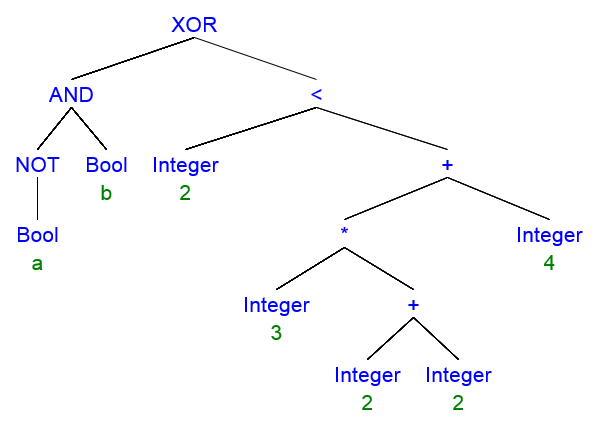
\includegraphics[width=0.7\textwidth]{Design/Expressions/precidenceExamples.png}
\caption{The parse tree for \textnormal{\enquote{$\Tnot a \Tand b \Txor 2 < 3 * (2 + 2) + 4$}}} %[XOR [AND [NOT [Bool a]][Bool b]] [< [Integer 2] [+ [* [Integer 3] [+ [Integer 2] [Integer 2]]] [Integer 4]]]]
\label{precedenceExamples}
\end{figure}

We can see that the operator placed lowest in the tree is \enquote{+} even though \enquote{*} has a lower precedence. This is done because the parentheses overwrites the the order so that everything inside gets higher precedence as intended. If we insert parentheses to illustrate the implicit precedence in the expression it would look like this:
\begin{center}
$((\Tnot a) \Tand b) \Txor (2 < ((3 * (2 + 2)) + 4))$
\end{center}
In \cref{precedenceExamples} we can see that the \enquote{XOR} operator is placed highest in the tree meaning that it has the lowest precedence. We can also see from the tree that this operator takes the result from \enquote{AND} and \enquote{<} as arguments where \enquote{<} again takes the result from \enquote{+} and the integer 2 as arguments and so on. We can see that the arguments changes type as we traverse the tree. We now look at the semantics and what impact this has on the formal type rules.

\subsection{Arithmetic Expressions}

First we look at arithmetic expressions. Arithmetic expressions are in TLDR defined as expressions that evaluates to a number, either a real or integer. The operators that creates the arithmetic expressions are +, -, *, /, \%, $\Tpot$ and \#. 

\begin{itemize}
\item "+" is a binary operator that adds two numbers of the same type

\begin{align*}
&\inference[$\text{ADD}_\text{L}$]{e \vdash a_1 \Rightarrow_A a_1'}
                    {e \vdash  a_1 + a_2 \Rightarrow_A a_1' + a_2}
&
&\inference[$\text{ADD}_\text{R}$]{e \vdash a_1 \Rightarrow_A a_1'}
                    {e \vdash a_2 + a_1 \Rightarrow_A a_2 + a_1'}
\\\\
&\inference[$\text{ADD}_\text{V}$]{}
                    {v_1 + v_2 \Rightarrow_A v}
                    {, v_1 + v_2 = v}
\end{align*}

\item "-" is a binary operator that subtracts two numbers of the same type

\begin{align*}
&\inference[$\text{SUB}_\text{L}$]{e \vdash a_1 \Rightarrow_A a_1'}
                    {e \vdash a_1 - a_2 \Rightarrow_A a_1' - a_2}
&
&\inference[$\text{SUB}_\text{R}$]{e \vdash a_1 \Rightarrow_A a_1'}
                    {e \vdash a_2 - a_1 \Rightarrow_A a_2 - a_1'}
\\\\
&\inference[$\text{SUB}_\text{V}$]{}
                    {v_1 - v_2 \Rightarrow_A v}
                    {, v_1 - v_2 = v}
\end{align*}

\item "*" is a binary operator that multiplies two numbers of the same type

\begin{align*}
&\inference[$\text{MULT}_\text{L}$]{e \vdash a_1 \Rightarrow_A a_1'}
                     {e \vdash a_1 * a_2 \Rightarrow_A a_1' * a_2}
&
&\inference[$\text{MULT}_\text{R}$]{e \vdash a_1 \Rightarrow_A a_1'}
                     {e \vdash a_2 * a_1 \Rightarrow_A a_2 * a_1'}
\\\\
&\inference[$\text{MULT}_\text{V}$]{}
                     {v_1 * v_2 \Rightarrow_A v}
                     {, v_1 * v_2 = v}
\end{align*}

\item "/" is a binary operator that divides two numbers of the same type

\begin{align*}
&\inference[$\text{DIV}_\text{L}$]{e \vdash a_1 \Rightarrow_A a_1'}
                    {e \vdash a_1 / a_2 \Rightarrow_A a_1' / a_2}
&
&\inference[$\text{DIV}_\text{R}$]{e \vdash a_1 \Rightarrow_A a_1'}
                    {e \vdash a_2 / a_1 \Rightarrow_A a_2 / a_1'}
\\\\
&\inference[$\text{DIV}_\text{V}$]{}
                    {v_1 / v_2 \Rightarrow_A v}
                    {, \frac{v_1}{v_2} = v}
\end{align*}

\item "\%" is a binary operator that returns the remainder of a floored division of two numbers of the same type

\begin{align*}
&\inference[$\text{MOD}_\text{L}$]{e \vdash a_1 \Rightarrow_A a_1'}
                    {e \vdash a_1 \% a_2 \Rightarrow_A a_1' \% a_2}
&
&\inference[$\text{MOD}_\text{R}$]{e \vdash a_1 \Rightarrow_A a_1'}
                    {e \vdash a_2 \% a_1 \Rightarrow_A a_2 \% a_1'}
\\\\
&\inference[$\text{MOD}_\text{V}$]{}
                    {v_1 \% v_2 \Rightarrow_A v}
                    {, v_1 \;\; \textrm{mod} \;\; v_2 = v}
\end{align*}

\item "\^{}" is a binary operator that lifts the first number to the power of the second number

\begin{align*}
&\inference[$\text{POW}_\text{L}$]{e \vdash a_1  \Rightarrow_A a_1'}
                    {e \vdash a_1 \Twedge a_2 \Rightarrow_A a_1' \Twedge a_2}
&
&\inference[$\text{POW}_\text{R}$]{e \vdash a_1 \Rightarrow_A a_1'}
                    {e \vdash a_2 \Twedge a_1 \Rightarrow_A a_2 \Twedge a_1'}
\\\\
&\inference[$\text{POW}_\text{V}$]{}
                    {v_1 \Twedge v_2 \Rightarrow_A v}
                    {, v_1 ^ {v_2} = v}
\end{align*}

\item "\#" is a binary operator that roots the first operand to the second operand
\begin{align*}
&\inference[$\text{ROOT}_\text{L}$]{e \vdash a_1 \Rightarrow_A a_1'}
                    {e \vdash a_1 \# a_2 \Rightarrow_A a_1' \# a_2}
&
&\inference[$\text{ROOT}_\text{R}$]{e \vdash a_1 \Rightarrow_A a_1'}
                    {e \vdash a_2 \# a_1 \Rightarrow_A a_2 \# a_1'}
\\\\
&\inference[$\text{ROOT}_\text{V}$]{}
                    {v_1 \# v_2 \Rightarrow_A v}
                    {, \sqrt[v_1]{v_2} = v}
\end{align*}

\item "( )" Parenteses gives what they surrounds the highest precedence.

\begin{align*}
&\inference[$\text{PARENS}_\text{A}$]{e \vdash a_1 \Rightarrow_A a_1'}
                       {e \vdash (a_1) \Rightarrow_A (a_1')}
&
&\inference[$\text{PARENS}_\text{V}$]{}
                       {(v) \Rightarrow_A v}
\end{align*}
\end{itemize}

For simplicity we create the following set since all type rules for these are the same.

\begin{center}
$\Taop = \left\{ {+, -, *, /, \%, \; \Tpot \;} \right\}$
\end{center}

Due to the semantics of all \enquote{AOP} operators these can not evaluate to a real if the two inputs are both integers. Therefore all operators in this set can take either two integers and evaluate to an integer or two reals and evaluate to a real. The operators cannot take a combination of real and iteger. This is done since all implicit type casts are avoided in TLDR. The reason for this is that the language is designed to give the programmer all errors as early as possible, preferably on compile-time, see \cref{typesys}. With no implicit type casts the programmer is always aware when type casts are performed and will therefore not be as prone to make runtime type errors.

The \enquote{\#} operator is a bit different. When taking the an integer root of another integer it can still evaluate to a real, for instance $\sqrt[2]{2} = $

This is formally

\begin{align*}
&\inference[$\text{EXPR}_{\Tint,\Tint}$]{\Tenv e_1  : \Tint & 
                       \Tenv e_2 : \Tint}
                    {\Tenv e_1 \mathbin{\text{op}} e_2 : \Tint},  \text{op} \in \Taop
%%%%%%%%%%%%%%%%%%%%%%%%%%%%%%%%%%%%%%%%%%%%%%%%%%%%%%%%%%%%%%%%%%%%%%%%%%%%%%%%%%%%%%%%
\\\\
&\inference[$\text{EXPR}_{\Treal,\Treal}$]{\Tenv e_1 : \Treal & 
                       \Tenv e_2 : \Treal}
                    {\Tenv e_1 \mathbin{\text{op}} e_2 : \Treal},  \text{op} \in \Taop
%%%%%%%%%%%%%%%%%%%%%%%%%%%%%%%%%%%%%%%%%%%%%%%%%%%%%%%%%%%%%%%%%%%%%%%%%%%%%%%%%%%%%%%%
\\\\
&\inference[$\text{ROOT}_{\Tint,\Tint}$]{\Tenv e_1 : \Tint &
                       \Tenv e_2 : \Tint}
                    {\Tenv e_1 \mathbin{\#} e_2 : \Treal}
%%%%%%%%%%%%%%%%%%%%%%%%%%%%%%%%%%%%%%%%%%%%%%%%%%%%%%%%%%%%%%%%%%%%%%%%%%%%%%%%%%%%%%%%
\\\\
&\inference[$\text{ROOT}_{\Treal,\Treal}$]{\Tenv e_1 : \Treal &
                       \Tenv e_2 : \Treal}
                    {\Tenv e_1 \mathbin{\#} e_2 : \Treal}
\end{align*}

\subsection{Boolean Expressions}
\begin{align*}
&\inference[$\text{BOOL}_{\Tbaop-\Tint,\Tint}$]{\Tenv e_1 : \Tint & 
                       \Tenv e_2 : \Tint}
                    {\Tenv e_1 \mathbin{\text{op}} e_2 : \Tbool}, \text{op} \in \Tbaop
%%%%%%%%%%%%%%%%%%%%%%%%%%%%%%%%%%%%%%%%%%%%%%%%%%%%%%%%%%%%%%%%%%%%%%%%%%%%%%%%%%%%%%%%
\\\\
&\inference[$\text{BOOL}_{\Tbaop-\Treal,\Treal}$]{\Tenv e_1 : \Treal &
                       \Tenv e_2 : \Treal}
                    {\Tenv e_1 \mathbin{\text{op}} e_2 : \Tbool}, \text{op} \in \Tbaop
%%%%%%%%%%%%%%%%%%%%%%%%%%%%%%%%%%%%%%%%%%%%%%%%%%%%%%%%%%%%%%%%%%%%%%%%%%%%%%%%%%%%%%%%
\\\\
&\inference[$\text{BOOL}_{EQUALS}$]{\Tenv e_1 : \Tt &
                       \Tenv e_2 : \Tt}
                    {\Tenv e_1 = e_2 : \Tbool}
%%%%%%%%%%%%%%%%%%%%%%%%%%%%%%%%%%%%%%%%%%%%%%%%%%%%%%%%%%%%%%%%%%%%%%%%%%%%%%%%%%%%%%%%
\\\\
&\inference[$\text{BOOL}_{NEQUALS}$]{\Tenv e_1 : \Tt &
                       \Tenv e_2 : \Tt}
                    {\Tenv e_1 \mathbin{\text{!=}} e_2 : \Tbool}
%%%%%%%%%%%%%%%%%%%%%%%%%%%%%%%%%%%%%%%%%%%%%%%%%%%%%%%%%%%%%%%%%%%%%%%%%%%%%%%%%%%%%%%%
\\\\
&\inference[$\text{BOOL}_{BBOP}$]{\Tenv e_1 : \Tbool &
                       \Tenv e_2 : \Tbool}
                    {\Tenv e_1 \mathbin{\text{op}} e_2 : \Tbool}, \text{op} \in \Tbop
%%%%%%%%%%%%%%%%%%%%%%%%%%%%%%%%%%%%%%%%%%%%%%%%%%%%%%%%%%%%%%%%%%%%%%%%%%%%%%%%%%%%%%%%
\\\\
&\inference[$\text{BOOL}_{NOT}$]{\Tenv e : \Tbool}
                    {\Tenv \mathbin{\text{NOT}} \; e : \Tbool}
\end{align*}

\begin{grammar}
<Operand>	::= <Block>
 \alt <Integer>
 \alt <Real>
 \alt <Boolean>
 \alt <Identifier>
 \alt <Literals>
 \alt <Invocation>

<Identifier> ::= 'me'
 \alt <Identifier>
 \alt <Identifier> <Accessor>
											
<Identifier> ::= [a-zA-Z][a-zA-Z\_0-9]*-('let' | 'var' | <Primitive> | 'struct' | 'actor' | 'receive' | 'send' | 'spawn' | 'wait' | 'return' | 'for' | 'in' | 'if' | 'else' | 'while' | 'die' | 'me')

<Accessor> ::= '.' <Identifier>
 \alt '.' '[' <Operation> ']'

<Primitive> ::= 'void' | 'int' | 'real' | 'char' | 'bool'

<Literals> ::= <String>
 \alt <ListRange>
 \alt <StructLiteral>
 \alt <Tuple>

<Boolean> ::= 'true' | 'false'

<Integer> ::= '-'?[1-9][0-9]* | '0'

<Real> ::= ([0-9]+'.'[0-9]+)|([0-9]+'.')|('.'([0-9])+)

<String> ::= '\textquotedbl' (U+0020 .. U+007E)* '\textquotedbl'

<Char> ::= '\textquotesingle' U+0020 .. U+007E '\textquotesingle'
\end{grammar}

The following mathematical operations are built into the language. They follow these semantic base rules:

\begin{align*}
&\inference[NUM]{}
                  {e \vdash n \Rightarrow_A v}
                  {, \mathcal{N}(n) = v}
\\\\
&\inference[$\text{INVOKE}_{A1}$]{\Braket{S,e} \Rightarrow_A v}
                  {\Braket{p,e} \Rightarrow_A v}
                  {,e(p) = \Braket{S,\epsilon}}
\\\\
&\inference[$\text{INVOKE}_{A2}$]{\Braket{S_1,e[p_1' \mapsto \Braket{S_2,p_2'}]} \Rightarrow_A v}
                  {\Braket{p_1(p_2),e} \Rightarrow_A v}
                  {,e(p_1) = \Braket{S_1,p_1'}, e(p_2) = \Braket{S_2,p_2'}}
\\\\
\end{align*}


\paragraph{Logical Operations}
\label{sec:logicOps}

For logical comparisons we chose \enquote{=}. This was done in accordance with the goal of keeping a natural mathematical language. In mathematics \enquote{=} is read as \enquote{is equal to} or simply \enquote{equals}, and is used for stating that two parts are equivalent to each other. Sometimes mathematicians use this statement in a contradicting manner, where they expect to prove the statement to be false. It is from this perspective of being a statement, either true or false, that we chose \enquote{=} to be a logical comparison. The same arguments exist for other types of logical operations.

\begin{itemize}
\item "=" is a binary operator that compares the two operands for equality. Returns true if equal. False otherwise.

\begin{align*}
&\inference[$\text{EQUALS}_\text{L}$]{e \vdash a_1 \Rightarrow_B a_1'}
                    {e \vdash a_1 = a_2 \Rightarrow_B a_1' = a_2}
&
&\inference[$\text{EQUALS}_\text{R}$]{e \vdash a_1 \Rightarrow_B a_1'}
                    {e \vdash a_2 = a_1 \Rightarrow_B a_2 = a_1'}
\\\\
&\inference[$\text{EQUALS}_\text{V1}$]{}
                    {v_1 = v_2 \Rightarrow_B \top}
                    {, v_1 = v_2}
&
&\inference[$\text{EQUALS}_\text{V2}$]{}
                    {v_1 = v_2 \Rightarrow_B \bot}
                    {, v_1 \neq v_2}
\\\\
&\inference[$\text{EQUALS}_\text{Actor}$]{a(act_1) = e\\ a(act_2) = e}
                    {act_1 = act_2 \Rightarrow_B \top}
&
&\inference[$\text{EQUALS}_\text{Actor}$]{a(act_1) = e\\ a(act_2) = e'}
                    {act_1 = act_2 \Rightarrow_B \bot}
                    {e \neq e'}
\end{align*}

\item "!=" is a binary operator that compares the two operands for equality. Returns true if not equal. False otherwise.

\begin{align*}
&\inference[$NEQUALS$]{}
                    {e \vdash a_1 != a_2 \Rightarrow_B \Tnot (a_1 = a_2)}
\end{align*}

\item "<" is a binary operator that compares the two operands. Returns true if the first operand is strictly less than the second operand. False otherwise.

\begin{align*}
&\inference[$\text{LT}_\text{L}$]{e \vdash a_1 \Rightarrow_A a_1'}
                    {e \vdash a_1 < a_2 \Rightarrow_A a_1' < a_2}
&
&\inference[$\text{LT}_\text{R}$]{e \vdash a_1 \Rightarrow_A a_1'}
                    {e \vdash a_2 < a_1 \Rightarrow_A a_2 < a_1'}
\\\\
&\inference[$\text{LT}_\text{V1}$]{}
                    {v_1 < v_2 \Rightarrow_B \top}
                    {, v_1 < v_2}
&
&\inference[$\text{LT}_\text{V2}$]{}
                    {v_1 < v_2 \Rightarrow_B \bot}
                    {, v_1 \geq v_2}
\end{align*}

\item "<=" is a binary operator that compares the two operands. Returns true if the first operand is less than or equal to the second operand. False otherwise.

\begin{align*}
&\inference[$LTEQ$]{}
                    {e \vdash a_1 <= a_2 \Rightarrow_A (a_1 < a_2) \Tor (a_1 = a_2)}
\end{align*}

\item ">" is a binary operator that compares the two operands. Returns true if the first operand is strictly greater than the second operand. False otherwise.

\begin{align*}
&\inference[$\text{GT}_\text{L}$]{e \vdash a_1 \Rightarrow_A a_1'}
                    {e \vdash a_1 > a_2 \Rightarrow_A a_1' > a_2}
&
&\inference[$\text{GT}_\text{R}$]{e \vdash a_1 \Rightarrow_A a_1'}
                    {e \vdash a_2 > a_1 \Rightarrow_A a_2 > a_1'}
\\\\
&\inference[$\text{GT}_\text{V1}$]{}
                    {v_1 > v_2 \Rightarrow_B \top}
                    {, v_1 > v_2}
&
&\inference[$\text{GT}_\text{V2}$]{}
                    {v_1 > v_2 \Rightarrow_B \bot}
                    {, v_1 \leq v_2}
\end{align*}

\item ">=" is a binary operator that compares the two operands. Returns true if the first operand is greater than or equal to the second operand. False otherwise.

\begin{align*}
&\inference[$GTEQ$]{}
                    {e \vdash a_1 >= a_2 \Rightarrow_A (a_1 > a_2) \Tor (a_1 = a_2)}
\end{align*}
\end{itemize}

\paragraph{Boolean Operations}
\label{sec:boolOps}

The following operations only operate on bool types.

\begin{align*}
&\inference[$\text{INVOKE}_{B1\top}$]{\Braket{S,e} \Rightarrow_B \top}
                  {\Braket{p_1,e} \Rightarrow_B \top}
                  {,e(p) = \Braket{S,\epsilon}}
\\\\
&\inference[$\text{INVOKE}_{B1\bot}$]{\Braket{S,e} \Rightarrow_B \bot}
                  {\Braket{p_1,e} \Rightarrow_B \bot}
                  {,e(p) = \Braket{S,\epsilon}}
\\\\
&\inference[$\text{INVOKE}_{B2\top}$]{\Braket{S_1,e[p_1' \mapsto \Braket{S_2,p_2'}]} \Rightarrow_B \top}
                  {\Braket{p_1(p_2),e} \Rightarrow_B \top}
\\                  
&                 {,e(p_1) = \Braket{S_1,p_1'}, e(p_2) = \Braket{S_2,p_2'}}
\\\\
&\inference[$\text{INVOKE}_{B2\bot}$]{\Braket{S_1,e[p_1' \mapsto \Braket{S_2,p_2'}]} \Rightarrow_B \bot}
                  {\Braket{p_1(p_2),e} \Rightarrow_B \bot}
\\                  
&                 {,e(p_1) = \Braket{S_1,p_1'}, e(p_2) = \Braket{S_2,p_2'}}
\\\\
&\inference[$\text{PARENS}_\text{B}$]{e \vdash b_1 \Rightarrow_B b_1'}
                       {e \vdash (b_1) \Rightarrow_B (b_1')}
\end{align*}

\begin{itemize}
\item "AND" is a binary operator that returns true if both values are true. False otherwise

\begin{align*}
&\inference[$\text{AND}_1$]{e \vdash b_1 \Rightarrow_B \bot}
                    {e \vdash b_1 \Tand b_2 \Rightarrow_B \bot}
\\\\
&\inference[$\text{AND}_2$]{e \vdash b_1 \Rightarrow_B \top \\ b_2 \Rightarrow_B \bot}
                    {e \vdash b_1 \Tand b_2 \Rightarrow_B \bot}
\\\\
&\inference[$\text{AND}_3$]{e \vdash b_1 \Rightarrow_B \top \\ b_2 \Rightarrow_B \top}
                    {e \vdash b_1 \Tand b_2 \Rightarrow_B \top}
\end{align*}


\item "OR" is a binary operator that returns true if at least one value is true. False otherwise

\begin{align*}
&\inference[OR]{}
                 {e \vdash b_1 \Tor b_2 \Rightarrow_B \Tnot(\Tnot b_1 \Tand \Tnot b_2)}
\end{align*}

\item "XOR" is a binary operator that returns true if only one operand is true. False otherwise

\begin{align*}
&\inference[XOR]{}
                  {e \vdash b_1 \Txor b_2 \Rightarrow_B (\Tnot(b_1 \Tand b_2)) \Tand (b_1 \Tor b_2)}
\end{align*}

\item "NOR" is OR negated.

\begin{align*}
&\inference[NOR]{}
                   {e \vdash b_1 \Tnor b_2 \Rightarrow_B \Tnot( b_1 \Tor b_2 )}
\end{align*}

\item "NOT" is a unary operator that returns the opposite value of the operand.

\begin{align*}
&\inference[$\text{NOT}_\top$]{e \vdash b_1 \Rightarrow_B \top}
                       {e \vdash \Tnot b_1 \Rightarrow_B \bot}
\\\\
&\inference[$\text{NOT}_\bot$]{e \vdash b_1 \Rightarrow_B \bot}
                       {e \vdash \Tnot b_1 \Rightarrow_B \top}
\end{align*}

\item "NAND" is a binary operator that returns true if none or a single operand is true. False otherwise.

\begin{align*}
&\inference[NAND]{}
                   {e \vdash b_1 \Tnand b_2 \Rightarrow_B \Tnot( b_1 \Tand b_2 )}
\end{align*}

\end{itemize}


\paragraph{Loop Expressions}
\begin{align*}
\intertext{The conditional body of the while construct must be of type bool. The body of the while-loop can be of any type defined in $\Tt$}
&\inference[WHILE]{\Tenv b : \Tbool &
                  \Tenv e : \Tt}
                 {\Tenv \mathbin{\text{while}} \; (b) \; {e}: ok}
%%%%%%%%%%%%%%%%%%%%%%%%%%%%%%%%%%%%%%%%%%%%%%%%%%%%%%%%%%%%%%%%%%%%%%%%%%%%%%%%%%%%%%%%
\intertext{For loops can only work on lists. The counter variable is the type of a element in the list being iterated.}
&\inference[FOR]{\Tenv l : [\Tpt]}
                 {\Tenv \mathbin{\text{for}} \; \mathbin{\text{x}} \; \mathbin{\text{in}} \; {l} \; : ok },	 \Tenv x : \Tpt
\end{align*}

\paragraph{Comparison of structs}
\begin{align*}
%%%%%%%%%%%%%%%%%%%%%%%%%%%%%%%%%%%%%%%%%%%%%%%%%%%%%%%%%%%%%%%%%%%%%%%%%%%%%%%%%%%%%%%%
\intertext{}
&\inference[STRUCT]{\Tenv e_1: \Tt & \Tenv e_2: \Tt}
                 {\Tenv e_1 = e_2: \Tbool}
\end{align*}

\paragraph{Misc constructs}
\begin{align*}
\intertext{}
&\inference[BLOCK]{\Tenv s_1: \Tt & \Tenv s_2: \Tt'}
                 {\Tenv \{s_1; s_2\} : \Tt'}
%%%%%%%%%%%%%%%%%%%%%%%%%%%%%%%%%%%%%%%%%%%%%%%%%%%%%%%%%%%%%%%%%%%%%%%%%%%%%%%%%%%%%%%%
\intertext{}
&\inference[LET]{}
                 {\Tenv \mathbin{\text{let}} \; e:T: ok}
        %%%%%%%%%%%%%%%%%%%%%%%%%%%%%%%%%%%%%%%%%%%%%%%%%%%%%%%%%%%%%%%%%%%%%%%%%%%%%%%%%%%%%%%%
\intertext{}
&\inference[VAR]{}
                 {\Tenv \mathbin{\text{var}} \; e:T: ok}
                 %%%%%%%%%%%%%%%%%%%%%%%%%%%%%%%%%%%%%%%%%%%%%%%%%%%%%%%%%%%%%%%%%%%%%%%%%%%%%%%%%%%%%%%%
\intertext{}
&\inference[LET1]{\Tenv e_1: \Tt & \Tenv e_2: \Tt}
                 {\Tenv \mathbin{\text{let}} \; e_1 := e_2: ok}
        %%%%%%%%%%%%%%%%%%%%%%%%%%%%%%%%%%%%%%%%%%%%%%%%%%%%%%%%%%%%%%%%%%%%%%%%%%%%%%%%%%%%%%%%
\intertext{}
&\inference[VAR1]{\Tenv e_1: \Tt & \Tenv e_2: \Tt}
                 {\Tenv \mathbin{\text{var}} \; e_1 := e_2: ok}
                        %%%%%%%%%%%%%%%%%%%%%%%%%%%%%%%%%%%%%%%%%%%%%%%%%%%%%%%%%%%%%%%%%%%%%%%%%%%%%%%%%%%%%%%%
\intertext{}
&\inference[NUM]{\Tenv n:\Tint}
                 {\Tenv n: \Tint} 
                        %%%%%%%%%%%%%%%%%%%%%%%%%%%%%%%%%%%%%%%%%%%%%%%%%%%%%%%%%%%%%%%%%%%%%%%%%%%%%%%%%%%%%%%%
\intertext{}
&\inference[NUM1]{\Tenv n_1:\Tint & \Tenv n_2:\Tint}
                 {\Tenv n_1.n_2: \Treal}    
%%%%%%%%%%%%%%%%%%%%%%%%%%%%%%%%%%%%%%%%%%%%%%%%%%%%%%%%%%%%%%%%%%%%%%%%%%%%%%%%%%%%%%%%
\intertext{}
&\inference[INVOKE]{\Tenv n: \Tt}
                 {\Tenv n: \Tt}
\end{align*}
